\documentclass[aspectratio=169,11pt]{beamer}
\usepackage[T1]{fontenc}
\usepackage{lmodern,amsmath,amssymb,mathtools,bm,booktabs,array,graphicx,tikz}
\usetikzlibrary{arrows.meta,positioning,calc,decorations.pathreplacing,patterns}
\definecolor{ink}{HTML}{17344D}\definecolor{accent}{HTML}{087E8B}\definecolor{pale}{HTML}{EDF5F5}\definecolor{gold}{HTML}{AD6B19}
\providecommand{\dd}{\,\mathrm{d}}\providecommand{\R}{\mathbb{R}}
\providecommand{\E}{\mathbb{E}}\providecommand{\Var}{\operatorname{Var}}
\providecommand{\Cov}{\operatorname{Cov}}\providecommand{\diag}{\operatorname{diag}}
\providecommand{\norm}[1]{\left\lVert#1\right\rVert}
\providecommand{\abs}[1]{\left|#1\right|}
\usefonttheme{professionalfonts}
\setbeamercolor{normal text}{fg=black,bg=white}
\setbeamercolor{frametitle}{fg=ink,bg=white}
\setbeamercolor{title}{fg=ink}\setbeamercolor{structure}{fg=accent}
\setbeamercolor{block title}{fg=ink,bg=pale}\setbeamercolor{block body}{fg=black,bg=pale!40}
\setbeamercolor{alerted text}{fg=accent}
\setbeamerfont{frametitle}{size=\Large,series=\bfseries}
\setbeamerfont{title}{size=\LARGE,series=\bfseries}
\setbeamertemplate{navigation symbols}{}
\setbeamersize{text margin left=.7cm,text margin right=.7cm}
\setbeamertemplate{frametitle}{\vspace{.18cm}\insertframetitle\par\vspace{.1cm}{\color{accent}\hrule height .6pt}\vspace{.12cm}}
\newcommand{\notestarget}{notes.pdf}\newcommand{\noteslabel}{Notes}
\setbeamertemplate{footline}{\hspace{.7cm}\color{ink}\scriptsize Computational Cardiology\quad\href{\notestarget}{\noteslabel}\hfill\insertframenumber\,/\,\inserttotalframenumber\hspace{.7cm}\vspace{.18cm}}
\setbeamercovered{invisible}
\hypersetup{pdfauthor={Zan Ahmad},pdftitle={Rigid alignment and arclength representations of closed curves},pdfpagemode=UseNone}
\begin{document}
\begin{frame}[plain]\vfill
{\small\color{accent} Computational Cardiology \quad Lecture 13}\par\medskip
{\raggedright\hyphenpenalty=10000\exhyphenpenalty=10000\LARGE\bfseries\color{ink} Rigid alignment and arclength representations of closed curves}\par\bigskip
Zan Ahmad\par\smallskip
{\small Fall 2024}\par\vfill\end{frame}
\renewcommand{\notestarget}{notes.pdf\#note-ordered-polygonal-representations}
\begin{frame}[t,fragile,label=slide-a-cyclic-polygon-in-physical-coordinates]{A cyclic polygon in physical coordinates}
\[X=(x_0,\ldots,x_{n-1}),\qquad x_j\in\mathbb R^2\ \mathrm{mm}.\]\pause{} The final edge joins $x_{n-1}$ to $x_0$ without duplicating the first row.
\end{frame}
\renewcommand{\notestarget}{notes.pdf\#note-physical-size-and-pose-invariance}
\begin{frame}[t,fragile,label=slide-corresponding-point-rms]{Corresponding-point RMS}
\[d_{\rm RMS}(X,Y)=\left(\frac1n\sum_j\|x_j-y_j\|^2\right)^{1/2}.\]\pause{} Division by $n$ does not repair an incorrect correspondence.
\end{frame}
\renewcommand{\notestarget}{notes.pdf\#note-physical-size-and-pose-invariance}
\begin{frame}[t,fragile,label=slide-the-transformations-removed]{The transformations removed}
\[Y\mapsto YR+\boldsymbol1t,\qquad R^{\mathsf T}R=I,\quad\det R=1.\]\pause{} Physical scale and reflection are retained.
\end{frame}
\renewcommand{\notestarget}{notes.pdf\#note-physical-size-and-pose-invariance}
\begin{frame}[t,fragile,label=slide-eliminate-the-translation]{Eliminate the translation}
\[X_c=X-\boldsymbol1\bar x,\quad Y_c=Y-\boldsymbol1\bar y,\quad t=\bar x-\bar yR.\]\pause{} The vertex centroid depends on sampling density.
\end{frame}
\renewcommand{\notestarget}{notes.pdf\#note-the-proper-orthogonal-procrustes-problem}
\begin{frame}[t,fragile,label=slide-expand-the-least-squares-objective]{Expand the least-squares objective}
\[\|X_c-Y_cR\|_F^2=\|X_c\|_F^2+\|Y_c\|_F^2-2\operatorname{tr}(R^{\mathsf T}Y_c^{\mathsf T}X_c).\]\pause{} Only the final term depends on $R$.
\end{frame}
\renewcommand{\notestarget}{notes.pdf\#note-the-proper-orthogonal-procrustes-problem}
\begin{frame}[t,fragile,label=slide-the-cross-product-matrix]{The cross-product matrix}
\[Y_c^{\mathsf T}X_c=U\Sigma V^{\mathsf T}.\]\pause{} The singular vectors identify the best paired orientation in this two-dimensional problem.
\end{frame}
\renewcommand{\notestarget}{notes.pdf\#note-the-proper-orthogonal-procrustes-problem}
\begin{frame}[label=slide-enforce-a-proper-rotation-panel-1]{Before alignment}
\centering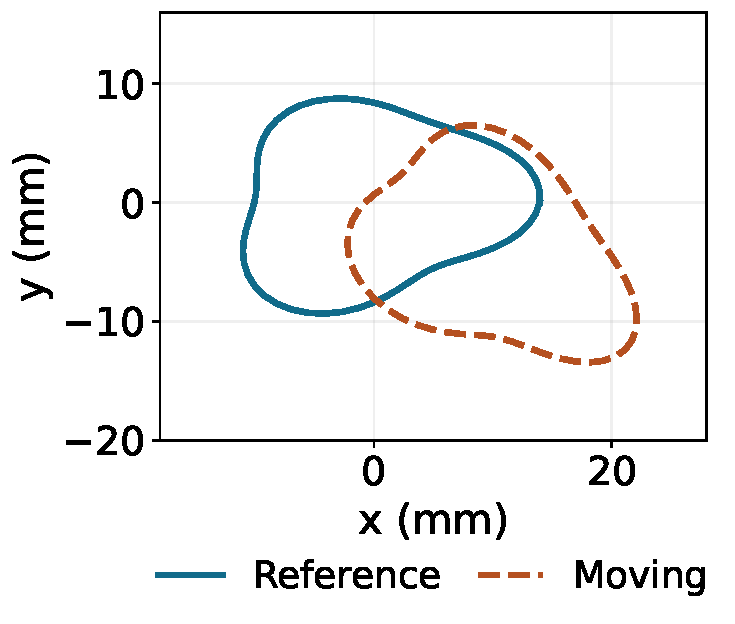
\includegraphics[width=.98\linewidth,height=.69\textheight,keepaspectratio]{presentation-figures/pose-alignment-panel-1.pdf}\end{frame}
\renewcommand{\notestarget}{notes.pdf\#note-the-proper-orthogonal-procrustes-problem}
\begin{frame}[label=slide-enforce-a-proper-rotation-panel-2]{Proper rigid alignment}
\centering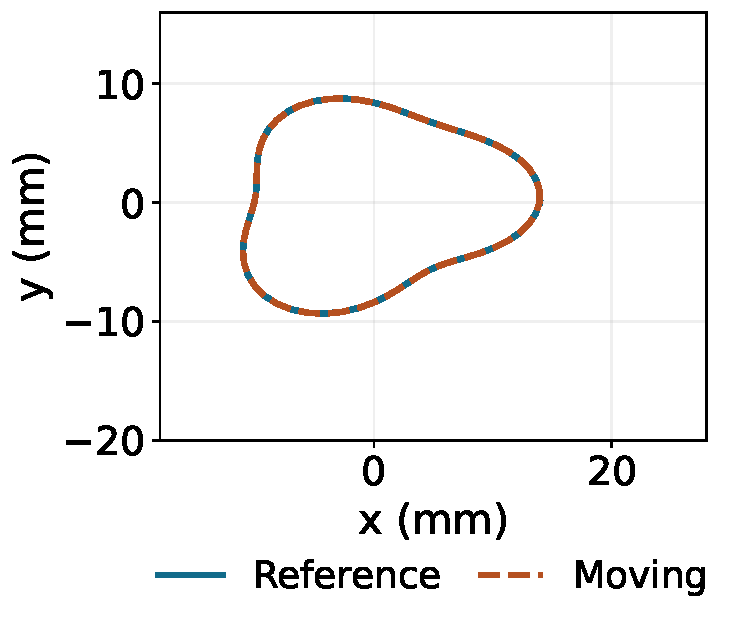
\includegraphics[width=.98\linewidth,height=.69\textheight,keepaspectratio]{presentation-figures/pose-alignment-panel-2.pdf}\end{frame}
\renewcommand{\notestarget}{notes.pdf\#note-the-proper-orthogonal-procrustes-problem}
\begin{frame}[t,fragile,label=slide-enforce-a-proper-rotation]{Enforce a proper rotation}
\[R=U\operatorname{diag}(1,\det(UV^{\mathsf T}))V^{\mathsf T}.\]\pause{} The determinant correction excludes a mirror transformation.
\end{frame}
\renewcommand{\notestarget}{notes.pdf\#note-physical-size-and-pose-invariance}
\begin{frame}[t,fragile,label=slide-retaining-physical-size]{Retaining physical size}
For centered, consistently oriented points,\[d_{\rm RMS}(X,aX)=|1-a|\left(\frac1n\sum_j\|x_j\|^2\right)^{1/2}.\]\pause{} Rigid alignment does not normalize scale.
\end{frame}
\renewcommand{\notestarget}{notes.pdf\#note-equal-arclength-resampling}
\begin{frame}[t,fragile,label=slide-point-density-changes-index-correspondence]{Point density changes index correspondence}
Equal-length arrays can sample different positions along the same curve.\pause{} A vertex index is not automatically a common anatomical location.
\end{frame}
\renewcommand{\notestarget}{notes.pdf\#note-equal-arclength-resampling}
\begin{frame}[t,fragile,label=slide-cumulative-polygonal-arclength]{Cumulative polygonal arclength}
\[s_k=\sum_{j<k}\|p_{j+1}-p_j\|,\qquad L=\sum_{j=0}^{n-1}\|p_{j+1}-p_j\|.\]\pause{} The sums include the closing edge.
\end{frame}
\renewcommand{\notestarget}{notes.pdf\#note-equal-arclength-resampling}
\begin{frame}[t,fragile,label=slide-equal-distance-targets]{Equal-distance targets}
\[q_\ell=\ell L/n,\qquad\ell=0,\ldots,n-1.\]\pause{} The target $L$ is excluded because it duplicates the start.
\end{frame}
\renewcommand{\notestarget}{notes.pdf\#note-equal-arclength-resampling}
\begin{frame}[label=slide-interpolate-within-an-edge-panel-1]{Same analytic contour}
\centering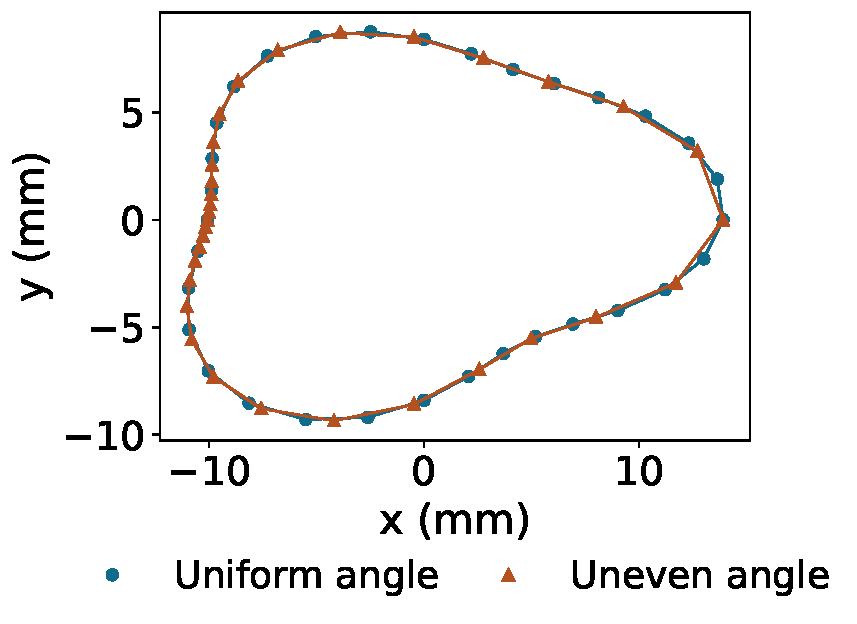
\includegraphics[width=.98\linewidth,height=.69\textheight,keepaspectratio]{presentation-figures/sampling-artifact-panel-1.pdf}\end{frame}
\renewcommand{\notestarget}{notes.pdf\#note-equal-arclength-resampling}
\begin{frame}[label=slide-interpolate-within-an-edge-panel-2]{Sampling artifact}
\centering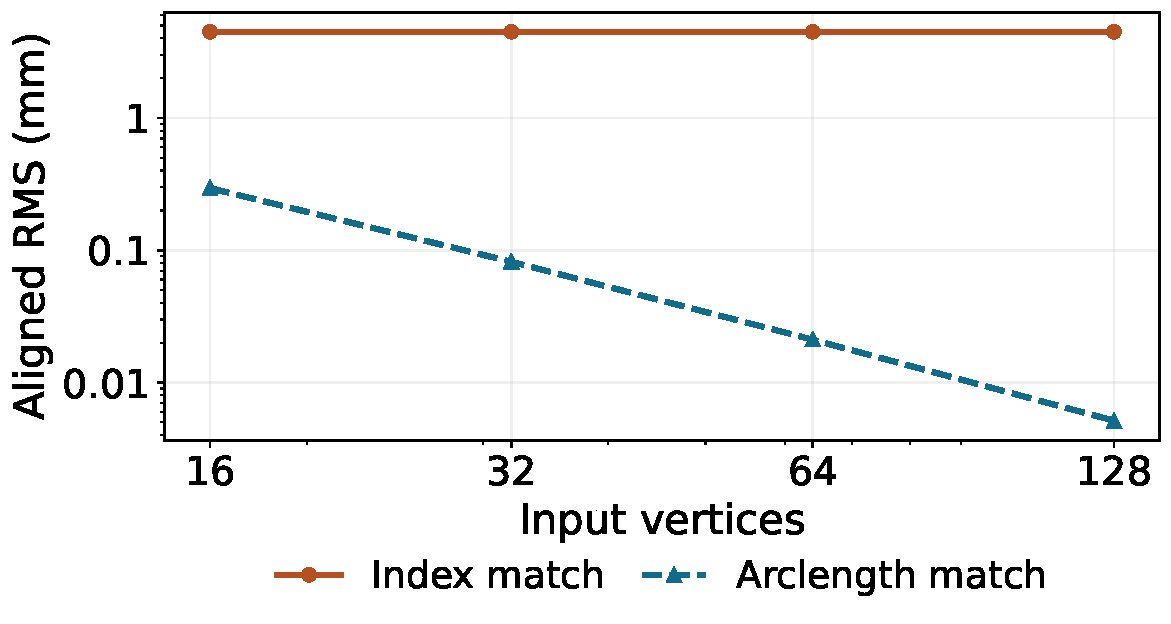
\includegraphics[width=.98\linewidth,height=.69\textheight,keepaspectratio]{presentation-figures/sampling-artifact-panel-2.pdf}\end{frame}
\renewcommand{\notestarget}{notes.pdf\#note-equal-arclength-resampling}
\begin{frame}[t,fragile,label=slide-interpolate-within-an-edge]{Interpolate within an edge}
\[\alpha=\frac{q-s_k}{s_{k+1}-s_k},\qquad x(q)=(1-\alpha)p_k+\alpha p_{k+1}.\]\pause{} Interpolation cannot recover an unresolved bend.
\end{frame}
\renewcommand{\notestarget}{notes.pdf\#note-degeneracies-and-retained-geometric-differences}
\begin{frame}[t,fragile,label=slide-zero-length-edges-and-zero-spread]{Zero-length edges and zero spread}
A repeated adjacent vertex creates a zero interpolation interval.\pause{} A zero-spread point set contains no orientation information.
\end{frame}
\renewcommand{\notestarget}{notes.pdf\#note-degeneracies-and-retained-geometric-differences}
\begin{frame}[t,fragile,label=slide-nonunique-alignment]{Nonunique alignment}
A degenerate cross-product matrix can make the minimizing rotation nonunique.\pause{} A minimizing transformation describes the stated paired coordinates; it does not establish anatomical correspondence.
\end{frame}
\renewcommand{\notestarget}{notes.pdf\#note-correspondence-and-the-meaning-of-a-residual}
\begin{frame}[t,fragile,label=slide-residual-components]{Residual components}
After pose removal, a discrepancy may reflect size, local deformation, sampling or segmentation.\pause{} Arclength fractions supply boundary positions, not validated landmarks.
\end{frame}
\end{document}
